\documentclass{article}
\usepackage{geometry}
\usepackage{paralist}
\usepackage[T1]{fontenc}
\usepackage{reledmac}
\usepackage{changepage}
\usepackage{layout}

\usepackage{multirow}

\usepackage{pgfplots}
\usepackage{tikz}
\usetikzlibrary{positioning}
\usetikzlibrary{shapes.geometric, arrows}
\usetikzlibrary{calc, shapes, backgrounds}
\tikzstyle{arrow} = [thick,->,>=stealth]

\usepackage{graphicx} 
\graphicspath{ {./images/} }

\usepackage{fancyhdr}
\fancyhead[L]{
	\begin{tabular}{l}
		\Large \textbf{\textsc{Advanced Networking and Future Internet}} \\
		\large Theoretical Exercise 10
	\end{tabular}
}
\fancyhead[R]{
	\begin{tabular}{r}
		16-124-836 \\
		Marcel \textsc{Zauder}
	\end{tabular}
}
\renewcommand{\headrulewidth}{0.4pt}
\fancyfoot[C]{\thepage}
\renewcommand{\footrulewidth}{0.4pt}
\setlength{\headsep}{35pt}
\setlength{\textheight}{600pt}

\usepackage{hyperref}

\begin{document}
	\pagestyle{fancy}
	
	\section*{10.1 Why are Special Encoding and the use of Zig-Zag Order necessary for the compression? Would the compression be possible using only DCT and Quantization?}
	\begin{adjustwidth}{2em}{2em}
		A good example for lossless data compression would be the entropy encoding which is used for compressing a JPEG image. The image components are arranged in a zig-zag order to be able to run the RLE (run-length encoding) algorithm which groups similar frequencies together, length codes the zeros and uses the Huffman coding algorithm for the rest. The RLE is a lossless data compression form which stores sequences in which the same data value occurs in consecutive data elements in single data values. Therefore the more runs are made the less the file size might become. The Huffman or arithmetic encoding is then used to encode the values to binary dependent on the occurrance frequency, meaning the more a value is occurring the less bits are used to encode it. \\
		A compression without zig-zag order or other special encoding methods would lead to many redundant values, which would lead to a still lossless compression but the file would be much larger.
	\end{adjustwidth}
	
	\section*{10.2 Different Encoding Algorithms}
	\begin{adjustwidth}{2em}{2em}
		\subsection*{10.2.1 Huffman Encoding Representation}
		\begin{adjustwidth}{2em}{2em}
			\begin{tabular}{ccc}
				\begin{tabular}{|r|r|}
					\hline
					\textbf{Symbol} & \textbf{Frequency} \\
					\hline
					E & 22 \\
					N & 14 \\
					A & 13 \\
					D & 12 \\
					V & 10 \\
					C & 9 \\
					T & 8 \\
					K & 7 \\
					I & 6 \\
					G & 5 \\
					'space' & 4 \\
					W & 3 \\
					O & 2 \\
					R & 1 \\
					\hline		
				\end{tabular}
				&
				&
				\begin{tabular}{|r|r|}
					\hline
					\textbf{Symbol} & \textbf{Encoding} \\
					\hline		
					V & 111 \\
					D & 110 \\
					A & 101 \\
					N & 010 \\
					E & 001 \\
					I & 1001 \\
					K & 0111 \\
					T & 0110 \\
					C & 0001 \\
					W & 10001 \\
					'space' & 00001 \\
					G & 00000 \\
					R & 100001 \\
					O & 100000 \\		
					\hline
				\end{tabular}
			\end{tabular}
			\newpage
			\textbf{Tree:} \\
			\begin{tikzpicture}[
    			scale = 1, transform shape, thick, every node/.style = {draw, circle, minimum size = 5mm},
    			grow = down,  % alignment of characters
    			level 1/.style = {sibling distance=6cm},
    			level 2/.style = {sibling distance=2cm}, 
    			level 3/.style = {sibling distance=1cm},
    			level 4/.style = {sibling distance=1cm}, 
    			level 5/.style = {sibling distance=1cm},
    			level 6/.style = {sibling distance=1cm},
    			level distance = 1.25cm
  			]
  				\node[fill = gray!40, shape = circle, minimum width = 1cm, font = \sffamily] (116) {116}
  				child { node[shape = circle, draw, line width=1pt, minimum size=8mm, inner sep=0mm] (69) {69}
  					child { node [] (40) {40}
  						child { node [] (18) {18}
  							child { node [] (9) {9}
  								child { node [] (G) {G} }
  								child { node [] (_) {\_} }
  							}
  							child { node [] (C) {C} }
  						}
  						child { node [] (E) {E} }
  					}
  					child { node [] (29) {29}
  						child { node [] (N) {N}	}
  						child { node [] (15) {15}
  							child { node [] (T) {T} }
  							child { node [] (K) {K} }
  						}
  					}
  				}
  				child {node[shape = circle, draw, line width=1pt, minimum size=10mm, inner sep=0mm] (47) {47}
  					child { node [] (25) {25}
  						child { node [] (12) {12}
  							child { node [] (6) {6}
  								child { node [] (3) {3}
  									child { node [] (O) {O} }
  									child { node [] (R) {R} }
  								}
  								child { node [] (W) {W} }
  							}
  							child { node [] (I) {I} }
  						}
  						child { node [] (A) {A} }
  					}
  					child { node [] (22) {22}
  						child { node [] (D) {D} }
  						child { node [] (V) {V} }
  					}
  				};

  				% Labels
  				\begin{scope}[nodes = {draw = none}]
    				\path (116)-- (69) node [near start, left]  {$0$};
    				\path (116)-- (47) node [near start, right]  {$1$};
    				\path (69) -- (40) node [near start, left]  {$0$};
    				\path (69) -- (29) node [near start, right]  {$1$};
    				\path (47) -- (25) node [near start, left]  {$0$};
    				\path (47) -- (22) node [near start, right]  {$1$};
    				\path (40) -- (18) node [near start, left]  {$0$};
    				\path (40) -- (E) node [near start, right]  {$1$};
    				\path (29) -- (N) node [near start, left]  {$0$};
    				\path (29) -- (15) node [near start, right]  {$1$};
    				\path (25) -- (12) node [near start, left]  {$0$};
    				\path (25) -- (A) node [near start, right]  {$1$};
    				\path (22) -- (D) node [near start, left]  {$0$};
    				\path (22) -- (V) node [near start, right]  {$1$};
    				\path (18) -- (9) node [near start, left]  {$0$};
    				\path (18) -- (C) node [near start, right]  {$1$};
    				\path (15) -- (T) node [near start, left]  {$0$};
    				\path (15) -- (K) node [near start, right]  {$1$};
    				\path (12) -- (6) node [near start, left]  {$0$};
    				\path (12) -- (I) node [near start, right]  {$1$};
    				\path (9)  -- (G) node [near start, left]  {$0$};
    				\path (9)  -- (_) node [near start, right]  {$1$};
    				\path (6)  -- (3) node [near start, left]  {$0$};
    				\path (6)  -- (W) node [near start, right]  {$1$};
    				\path (3)  -- (O) node [near start, left]  {$0$};
    				\path (3)  -- (R) node [near start, right]  {$1$};
  				\end{scope}
			\end{tikzpicture}
		\end{adjustwidth}
		\subsection*{10.2.2 Arithmetic Encoding Representation}
		\begin{adjustwidth}{-2em}{}
			\begin{tabular}{|l|r|r|l|r|}
				\hline
				\multirow{2}{*}{\textbf{Symbol}} & \multirow{2}{*}{\textbf{Frequency}} & \textbf{Probability} & \multicolumn{2}{|c|}{\textbf{Interval reduced to ten-bit precision}} \\
				\cline{3-5}
				& & \textbf{(as fraction)} & \textbf{(as fractions)} & \textbf{(in binary)} \\
				\hline
				E & 22 & 22/116 & $[0, 194/1024)$ & $[0.0000000000, 0.0011000010)$ \\
				N & 14 & 14/116 & $[194/1024, 318/1024)$ & $[0.0011000010, 0.0100111101)$ \\
				A & 13 & 13/116 & $[318/1024, 433/1024)$ & $[0.0100111101, 0.0110110000)$ \\
				D & 12 & 12/116 & $[433/1024, 538/1024)$ & $[0.0110110000, 0.1000011010)$ \\
				V & 10 & 10/116 & $[538/1024, 627/1024)$ & $[0.1000011010, 0.1001110011)$ \\
				C & 9 & 9/116 & $[627/1024, 706/1024)$ & $[0.1001110011, 0.1011000010)$ \\
				T & 8 & 8/116 & $[706/1024, 777/1024)$ & $[0.1011000010, 0.1100001001)$ \\
				K & 7 & 7/116 & $[777/1024, 839/1024)$ & $[0.1100001001, 0.1101000111)$ \\
				I & 6 & 6/116 & $[839/1024, 892/1024)$ & $[0.1101000111, 0.1101111100)$ \\
				G & 5 & 5/116 & $[892/1024, 936/1024)$ & $[0.1101111100, 0.1110101000)$ \\
				'space' & 4 & 4/116 & $[936/1024, 971/1024)$ & $[0.1110101000, 0.1111001011)$ \\
				W & 3 & 3/116 & $[971/1024, 998/1024)$ & $[0.1111001011, 0.1111100110)$ \\
				O & 2 & 2/116 & $[998/1024, 1015/1024)$ & $[0.1111100110, 0.1111110111)$ \\
				R & 1 & 1/116 & $[1015/1024, 1)$ & $[0.1111110111, 1.0000000000)$ \\
				\hline
			\end{tabular}
		\end{adjustwidth}
		\subsection*{10.2.3 How many bit are necessary to encode the string \\ "ADVANCED NETWORKING" under each encoding?}
		\begin{adjustwidth}{2em}{2em}
			In the arithmetic encoding only 10 bits are needed to encode the whole string, because this is the precision given for our arithmetic encoding. When using the Huffman-Encoding Algorithm in total "ADVANCED NETWORKING" is encoded to "101 110 111 110 010 0001 001 110 00001 010 001 0110 10001 100000 100001 0111 1001 010 00000" which has 73 bits.
		\end{adjustwidth}
	\end{adjustwidth}
	
	\section*{10.3 Traditional Video Encoding}
	\begin{adjustwidth}{2em}{2em}
		\subsection*{10.2.1 What are the roles of each type of frame in traditional video encoding (I, P, and B), and what kind of information is encoded in each of the types?}
		\begin{adjustwidth}{2em}{2em}
			I-frames (intra-coded pictures) is a complete image encoded without any reference to another frame; for example in JPEG for Y, Cb, Cr. The P-Frames holds information about the changes in the image from the previous frame. The data encoded are motion vectors for the prediction and transform coefficients for the prediction correction. The B-Frames holds information about the differences for both the previous and future frame.
		\end{adjustwidth}
		\subsection*{10.2.1 Different frame losses have different effects in overall video res-construction, what is the effect of loss of frames I, P, and B?}
		\begin{adjustwidth}{2em}{2em}
			When loosing an I-Frame the following P and B-Frames cannot be encoded. Also if in the I-Frame there is an error this will lead to errors in the corresponding P and B-Frames as well. To minimize this corruption probability the I-Frames must occur periodically. \\
			A loss of a P-Frame will lead to the following P and B-Frames not being able to be decoded. \\
			A loss of a B-Frame is the less concern because it only has information about itself, so any other previous and future frame can still be decoded.
		\end{adjustwidth}
	\end{adjustwidth}
	
	\section*{10.4 How can motion estimation be achieved with the use of Macro-Blocks (block-matching algorithm)?}
	\begin{adjustwidth}{2em}{2em}
		A macro-block is a combination of 4 blocks (8x8) for the Luminance Y, 1 block for Chromatic-red and 1 block for Chromatic-blue. Each of these macro-blocks is compared pixel-by-pixel with the corresponding macro-block of the preceding I or P-frame. The algorithm searches for similarities in the previous or future frame and if found the Macro-Block is encoded. If no close match is found the constraints are relaxed and in a limited area around this macro-blick another search is executed. If a match is found additionally to the Macro-Block encoding the motion vector and the prediction error are also encoded as well. Typically, only Y Luminance values are used for the motion estimation.
	\end{adjustwidth}
	
	\section*{10.5 Explain the components and steps in MPEG-1 encoding and decoding.}
	\begin{adjustwidth}{2em}{2em}
		\begin{enumerate}
			\item \textbf{Encoder} \\
			The first step for encoding is to calculate the difference between the current and previous frames. Additionally the frame is used for motion estimation \& compensation which searches for similar macro-blocks. After this the frame is put through the DCT and Quantization algorithm. This so prepared frame is then put through the invers for the synthetization-analysis concept in which it is preconstructed so it can be used for the motion estimation. Last the fram is encoded with entropy encoding.
			\item \textbf{Decoder} \\
			First the data is decoded with a similar entropy decoder and then the Quantization and DCT are reversed by using there inverse algorithm. In the motion compensation block we have a storage for the previous and future picture so the encoded frame can be reconstructed. The process of decoding is much easier than the encoding.
		\end{enumerate}
	\end{adjustwidth}
	
	\section*{10.6 Bonus Question}
	\begin{adjustwidth}{2em}{2em}
		\subsection*{10.6.1 Analyzing Outputs and Importance of each Step}
		\begin{adjustwidth}{2em}{2em}
			First the image is grayscaled because the luminance of an image is much more important than colors. Then the quantization is run. In there 8x8 blocks are extracted from the image and the DCT algorithm is run over them and then they are put together to create a whole dct image. This idct\_whole image is then used for the dequantization. In there the image is again split up in the 8x8 blocks and then are used in the inverse DCT algorithm to recreate the image. \\
			After the recreation the SSIM and PSNR values are computed by comparing the recreated and the initial image.
		\end{adjustwidth}
		\subsection*{10.6.2 Other Quantization Matrixes}
		\begin{adjustwidth}{2em}{2em}
			When using the qt\_y matrix we have the highest SSIM and PSNR values, therefore it is the most similar reconstructed image and the edges in the picture are very sharp. \\
			Using the qt\_cr matrix the results are pretty much the same as when we use the default matrix. Also the SSIM and PSNR values are similar to the ones the default matrix was generating. \\
			The qt\_cb matrix has the lowest values for both SSIM and PSNR. In the comparison image it can be seen when zooming into the reconstructed image. In there the edges between the eye and the face are a little bit more blurry than when comparing it with the reconstructed image when using the qt\_y matrix.
		\end{adjustwidth}
	\end{adjustwidth}
\end{document}